\documentclass{elsarticle} %review
\usepackage[english]{babel}

%%% functional packages
\usepackage{amssymb, mathtools, amsthm, mathrsfs}
\usepackage{subcaption}
\usepackage{graphicx}
\graphicspath{{_pics/}}

%%% configuration packages
\usepackage{fullpage}
\usepackage{comment}

\usepackage{xcolor}
\newcommand{\todo}[1]{\textcolor{olive}{#1}}
\newcommand{\alert}[1]{\textcolor{red}{\large \bf #1}}

% \usepackage{lineno}
% \modulolinenumbers[5]

\usepackage{hyperref}

\journal{Journal of \LaTeX\ Templates}

%%%%%%%%%%%%%%%%%%%%%%%
%% Elsevier bibliography styles
%%%%%%%%%%%%%%%%%%%%%%%
%% To change the style, put a % in front of the second line of the current style and
%% remove the % from the second line of the style you would like to use.
%%%%%%%%%%%%%%%%%%%%%%%

%% Numbered
%\bibliographystyle{model1-num-names}

%% Numbered without titles
%\bibliographystyle{model1a-num-names}

%% Harvard
%\bibliographystyle{model2-names.bst}\biboptions{authoryear}

%% Vancouver numbered
%\usepackage{numcompress}\bibliographystyle{model3-num-names}

%% Vancouver name/year
%\usepackage{numcompress}\bibliographystyle{model4-names}\biboptions{authoryear}

%% APA style
%\bibliographystyle{model5-names}\biboptions{authoryear}

%% AMA style
%\usepackage{numcompress}\bibliographystyle{model6-num-names}

%% `Elsevier LaTeX' style
\bibliographystyle{elsarticle-num}
%%%%%%%%%%%%%%%%%%%%%%%

% general
%\newcommand{\Kn}{\mathrm{Kn}}
\newcommand{\Ma}{\mathrm{Ma}}
\newcommand{\dd}{\mathrm{d}}
\newcommand{\pder}[2][]{\frac{\partial#1}{\partial#2}}
\newcommand{\pderdual}[2][]{\frac{\partial^2#1}{\partial#2^2}}
\newcommand{\pderder}[3][]{\frac{\partial^2#1}{\partial#2\partial#3}}
\newcommand{\pderderder}[4][]{\frac{\partial^3#1}{\partial#2\partial#3\partial#4}}
\newcommand{\Pder}[2][]{\partial#1/\partial#2}
\newcommand{\Pderdual}[2][]{\partial^2#1/\partial#2^2}
\newcommand{\Pderder}[3][]{\partial^2#1/\partial#2\partial#3}
\newcommand{\Set}[2]{\{\,{#1}:{#2}\,\}}
\newcommand{\OO}[1]{O(#1)}
\newcommand{\transpose}[1]{#1^\mathsf{T}}
\DeclarePairedDelimiter\autobracket()       % mathtools are needed
\newcommand{\br}[1]{\autobracket*{#1}}

\DeclareMathOperator{\sgn}{sgn}

% topic-specific
\newcommand{\dxi}{\dd{\boldsymbol{\xi}}}
\newcommand{\bxi}{\boldsymbol{\xi}}
\newcommand{\bpsi}{\boldsymbol{\psi}}
\newcommand{\bv}{\boldsymbol{v}}
\newcommand{\bq}{\boldsymbol{q}}
\newcommand{\bc}{\boldsymbol{c}}
\newcommand{\bn}{\boldsymbol{n}}
\newcommand{\be}{\boldsymbol{e}}
\newcommand{\bm}{\boldsymbol{m}}
\newcommand{\bT}{\boldsymbol{T}}
\newcommand{\bdot}{\boldsymbol{\cdot}}
\newcommand{\dx}{\dd{\boldsymbol{x}}}
\newcommand{\bx}{\boldsymbol{x}}
\newcommand{\equil}[1]{#1^\mathrm{(eq)}}
\newcommand{\refer}[1]{#1_0}
\newcommand{\LB}{\mathrm{LB}\!}
\newcommand{\DV}{\mathrm{DV}\!}

\newcommand{\xiai}{\xi_{j \alpha}}
\newcommand{\xiaj}{\xi_{j \beta}}
\newcommand{\xiak}{\xi_{j \gamma}}
\newcommand{\cai}{c_{j \alpha}}
\newcommand{\caj}{c_{j \beta}}
\newcommand{\cak}{c_{j \gamma}}
\newcommand{\ai}{a_{\alpha}}
\newcommand{\aij}{a_{\alpha\beta}}
\newcommand{\aijk}{a_{\alpha\beta\gamma}}
\newcommand{\Hi}{H_{\alpha}}
\newcommand{\Hij}{H_{\alpha\beta}}
\newcommand{\Hijk}{H_{\alpha\beta\gamma}}

\begin{document}

\begin{frontmatter}

\title{Kinetic multiscale scheme based on the discrete-velocity and lattice-Boltzmann methods}

\author[ccas]{V.V.~Aristov}
\author[ccas]{O.V.~Ilyin}
\author[skoltech,ccas]{O.A.~Rogozin\corref{cor}}
\cortext[cor]{Corresponding author}
\ead{oleg.rogozin@phystech.edu}

\address[ccas]{Dorodnicyn Computing Center,
    Federal Research Center "Computer Science and Control" of Russian Academy of Science, Moscow, Russia}
\address[skoltech]{Center for Design, Manufacturing, and Materials,
    Skolkovo Institute of Science and Technology, Moscow, Russia}

\begin{abstract}

A novel hybrid computational method based on the discrete-velocity (DV) approximation including the lattice-Boltzmann (LB) technique is proposed.
Numerical schemes for the kinetic equations are used in regions of rarefied flows and LB schemes are employed in continuum flow zones.
The schemes are written under the finite-volume (FV) formulation to achieve flexibility of local mesh refinement.
The expansion to the Hermite polynomials is used for the coupling of DV and LB solutions.
Special attention is paid to the recent high-order and regularized LB models.
The linear Couette flow is analyzed as a numerical example,
where a good correspondence with the benchmark solutions is obtained.
% [POISEUILLE]: The linear Couette and Poiseuille flows are analyzed as numerical examples,


%In the present paper, a novel hybrid fluid--kinetic computational approach based on the discrete-velocity (DV) approximation including lattice-Boltzmann (LB) technique is proposed. Numerical schemes for a kinetic equation are used in regions of rarefied flows and LB schemes are used in continuum flow zones. The problem devoted to matching solutions of DV and LB in buffer cells is solved using the expansion of the solutions of DV and LB models on Hermite polynomials and matching the expansion coefficients. A special attention is paid to the recent high-order LB models. Some variants of LBM are considered and the efficiency of the hybrid method is evaluated. The Couette-flow problem is investigated as a test. The criteria transformation from the continuum region to kinetic one is proposed and the influence of the point transformation is studied. The CPU times for the hybrid scheme and for BGK scheme are compared. The good correspondence with the benchmark solution is obtained: the computations on the basis of the hybrid method are close to the well-known tabulated solutions of the Couette flow.




\end{abstract}

\begin{keyword}
%kinetic--kinetic coupling,
%kinetic multiscale scheme,
hybrid numerical method,
discrete-velocity method,
lattice-Boltzmann method,
domain decomposition,
Knudsen layer.
\end{keyword}

\end{frontmatter}

% \linenumbers
\tableofcontents

\section{Introduction}\label{sec:intro}

%%% Effective numerical methods for multiscale problems
Thus far, effective numerical simulation of multiscale flows has remained a challenging problem despite the efforts of many researchers.
This is due, in particular, to complicated flow structures where small-scale highly nonequilibrium regions
coexist with large-scale equilibrium zones.
The use of the kinetic equation in all regions is very demanding from a computational point of view.
On the other hand, the computational fluid dynamics provide an efficient description of near-equilibrium flows,
but it is not adequate for regions where the velocity distribution function (VDF) is not close to Maxwellian
and the contribution of highest moments cannot be ignored.
% Therefore, computational fluid dynamics is being confronted with the challenge of constructing the unified numerical methods suitable for simulation of multiscale flows.
% The numerical solution of kinetic equations in stiff regimes represents a challenge in the construction of computational methods.
% one would like to avoid the expensive cost of solving the kinetic equation in regions well described by continuum fluid models,
% since the latter are easily solvable by classical numerical methods.
% Therefore, to strike a balance between computational costs and simulation accuracy,
% multiscale schemes are being developed that take advantage of both kinetic and continuum-fluid solvers,
% i.e., deploying a kinetic solver only in the rarefied flow regions and a continuum solver in the hydrodynamic regions.

%%% Hybrid schemes
There are two main approaches how to deal with the multiscale problems (see, e.g., review~\cite{Dimarco2014}).
The first one employs different kinds of representations for equilibrium and non-equilibrium parts of the solution
in the entire computational space, while the second one handles the problem by dividing the physical domain
into the highly rarefied and near-equilibrium regions using some criterion of domain decomposition.
The fluid--kinetic coupling is a natural and effective approach for the description of multiscale flows.
The coupling of the Boltzmann and Euler or Navier--Stokes (NS) equations
is a canonical example of such hybrid schemes (see, e.g.,~\cite{Bourgat1996, Tallec1997}).
%and has also been elaborated and applied within the Unified Flow Solver (UFS)~\cite{Kolobov2007}.
%1. Asymptotic-preserving schemes
%2. Dynamic domain decomposition strategies
%    A. Dynamic fluid--kinetic coupling methods:
%        a) A moving interface method: a stationary smooth transition strategy was proposed for this coupling.
%        b) A micro–macro moving interface method (Degond et al. 2010): micro–macro decomposition of the VDF
%3. Hybrid methods
%    A. Low-variance deviational Monte Carlo methods
%    % Variance reduction methods are a popular way to improve the accuracy of Monte Carlo methods by reducing the amount of fluctuations in the results (Caflisch 1998).
%    B. Moment-guided Monte Carlo methods
%    % The basic idea described here consists in obtaining reduced-variance Monte Carlo methods by forcing the statistical samples to match prescribed sets of moments given by the solution of deterministic macroscopic fluid equations (Degond et al. 2011, Dimarco 2013).
%    C. Hybrid multiscale methods (hybrid representation of the solution)
%    % different kind of representation of the solution as an equilibrium and non-equilibrium part, first introduced in Pareschi and Caflisch (1999).
%    % the solution in each cell is represented as a combination of two different parts, a stochastic particle representation of the non-equilibrium fraction and a deterministic representation of the equilibrium part

%%% Kinetic-based description of continuum media
We consider very briefly development and realization of these important ideas.
The kinetic-based description of continuum media has been suggested independently and has been widely used since the beginning of 80s,
see~\cite{Potkin1975, Pullin1980, Reitz1981, Aristov1983}. Later these kinetic-consistent schemes have been developed
in~\cite{Elizarova1985, Deshpande1986, Prendergast1993, Chou1997, Ohwada2004Xu, Ohwada2004Kobayashi, Ohwada2006}.
Such methods reproduce the Euler and NS dynamics.
The cellular-automata approximation for the NS equations was developed in the middle of 80s~\cite{Frisch1986}.
Finally, the lattice-gas model based on the BGK equation was proposed in the beginning of 90s~\cite{Qian1992}.
It gave rise to a wide class of numerical methods called lattice-Boltzmann (LB) methods~\cite{Higuera1989,Benzi1992,Succi2001}.
%%% Ilyin: Succi citation
The DV models of LB type which correctly decribe the hydrodynamic and non-hydrodynamic moments
up to the Burnett level were considered in~\cite{Xu2018, Xu2019}.

%%% Connection between DV and LB
It is worth emphasizing that there is a fundamental relationship between the LB and DV methods.
For instance, one can cite a phrase from~\cite{Rivet2001}:
``This type of discrete kinetic theory can be seen as the ancestor of the lattice gas approach''.
The LB method is genetically related to the Broadwell-type models~\cite{Broadwell1964shock, Gatignol1975},
which use a small number of discrete velocities to reproduce some relevant features of the Boltzmann equation.
Thus, the DV approximation is a natural basis for construction of a hybrid multiscale model.

%%% Known coupling schemes for LB
The mapping scheme for coupling the low-order and high-order LB models is presented in~\cite{Meng2011},
while the possibility of merging the DV and LB methods was noticed in~\cite{Succi2016}.
The methods of DSMC type in the kinetic zones and the Euler or NS equations in the continuum are well developed by now,
but the usual statistical modeling in the buffer zone yields some statistical noise especially for subsonic flows,
which complicates calculations.
This hybrid approach has been suggested in~\cite{Staso2016short, Staso2016long} and in the recent paper~\cite{Staso2018},
where the solution is obtained by means of coupling the DSMC and LB methods.
The first results on coupling of the LB an DV models for the one-dimensional case
based on matching of the half-fluxes have been presented in~\cite{Ilyin2018}.

%%% Why DV is better than DSMC?
Unlike DSMC, the methods of direct numerical solution of the Boltzmann equation do not give statistical noise of macroscopic parameters.
Therefore, hybrid methods based on a direct numerical solution of the Boltzmann equation appear to be more promising.
The DV schemes with the large number of discrete velocities are used in direct methods for solving BE, BGK, S-model or other kinetic equations.
The DV method is applied with the combination of Monte Carlo or quasi-Monte Carlo procedures for evaluating collision integrals
and for computing the appropriate moments which are used in the collision integrals of the model kinetic equations.
For the near-equilibrium zones, the small number of discrete velocities can be considered.
Therefore, one can expect that LB approaches are fit for describing flows in these regions.

%%% Our proposition
A novel hybrid kinetic approach for multiscale problems is proposed in this paper.
We attempt to couple the DV method for the Boltzmann equation (or its BGK model) and the LB method for the NS equations.
The DV method adequately describes nonequilibrium regions, while the LB one provides an adequate description in continuum regions.
To couple solutions between the DV and LB subdomains, we approximate the VDF by the truncated Hermite expansion in the buffer zone.
The high-order LB models~\cite{Shan2006, Feuchter2016}
% [POISEUILLE]: as well as the special regularization procedures~\cite{Latt2006, Mont2015}
are used to expand the continuum subdomain.

%%% FV formulation
The classical LB methods enjoy their efficiency as a result of highly symmetric discrete physical space and time.
However, uniform Cartesian grids lack flexibility and, therefore, local grid refinement.
There are several approaches how to work around this limitation.
The LB method is easily extended for arbitrary unstructured meshes
under the FV formulation~\cite{Succi1992, Peng1999, Patil2009, Li2016}.
In the present paper, this strategy is adopted, specifically to refine mesh near the boundary.

%%% Plan of the paper
The plan of the present paper is as follows.
The governing equations and nondimensional variables are introduced in Section~\ref{sec:equations}.
The mapping scheme is described in Section~\ref{sec:mapping}.
Details of the numerical methods used are presented in Section~\ref{sec:numerics}.
Section~\ref{sec:results} contains the numerical solutions of the Couette-flow problems, % [POISEUILLE]: Poiseuille-flow
obtained by the DV model, various LB models, and the proposed hybrid scheme,
as well as a discussion on the computational efficiency of the hybrid approach.
In section~\ref{sec:summary}, perspectives of the kinetic multiscale DV-LB methods are outlined.

\section{Main equations}\label{sec:equations}
%%%%%%%%%%%%%%%%%%%%%%%%%%%%%%%
%%% [Rogozin]: there should be nothing about Couette flow, discretization, methods, and algorithms in "Main equations"!
%%%%%%%%%%%%%%%%%%%%%%%%%%%%%%%

%%% Nondimensional variables
We first introduce the notation for describing a dilute gas.
Let \(L\), \(\refer\rho\), \(\refer{T}\), \(V = \sqrt{R\refer{T}}\) and \(\refer{p} = \refer{\rho}R\refer{T}\) be
the reference length, density, temperature, velocity, and pressure, respectively.
The specific gas constant \(R = k_B/m\), where \(k_B\) is the Boltzmann constant and \(m\) is the molar mass.
Then, \(f\refer{\rho}/V^3\) is the one-particle velocity distribution function (VDF)
defined in seven-dimensional space \((tL/V, \bx L, \bxi V)\) and
the macroscopic variables take the following form:
\(\rho\refer{\rho}\) is the density, \(\bv V\) is the velocity, \(T\refer{T}\) is the temperature,
\(p_{\alpha\beta}\refer{p}\) is the stress tensor, \(\bq\refer{p}V\) is the heat flux.
In the dimensionless form, they are calculated as polynomial moments of the VDF:
\begin{equation}\label{eq:macro}
    \begin{gathered}
    \rho = \int f \dxi, \quad
    \bv = \frac1{\rho} \int \bxi f \dxi, \quad
    T = \frac{1}{3\rho}\int|\bxi-\bv|^2f \dxi = \frac{p_{\alpha\alpha}}{3\rho}, \\
    p_{\alpha\beta} = \int(\xi_{\alpha}-v_{\alpha})(\xi_{\beta}-v_{\beta}) f \dxi, \quad
    \bq = \frac12\int(\bxi-\bv)|\bxi-\bv|^2 f \dxi.
    \end{gathered}
\end{equation}
Integration with respect to \(\bxi\) is, hereafter, carried out over \(\mathbb{R}^3\).

%%% Boltzmann equation
The VDF is governed by the Boltzmann equation
\begin{equation}\label{eq:Boltzmann}
    \pder[f]{t} + \bxi\bdot\pder[f]{\bx} = \frac1kJ(f),
\end{equation}
where \(J(f)\) is the collisional operator with a local Maxwellian as the equilibrium function
\begin{equation}\label{eq:equilibrium}
    \equil{f}\br{\bxi; \rho, \bv, T} = \frac{\rho}{(2\pi T)^{3/2}}\exp\br{-\frac{|\bxi-\bv|^2}{2T}}.
\end{equation}
The Knudsen number \(k\) can be expressed in terms of the reference gas viscosity \(\refer\mu\)~\cite{Sharipov1998}:
\begin{equation}\label{eq:Knudsen_number}
    k = \frac{\refer\mu V}{\refer{p}L}.
\end{equation}

%%% BGK equation
In the present paper, we restrict ourselves to the simplest relaxation model~\cite{Krook1954, Welander1954}
\begin{equation}\label{eq:bgk_integral}
    J(f)(\bxi) = \rho\br{\equil{f}(\bxi) - f(\bxi)},
\end{equation}
often referred as the Bhatnagar--Gross--Krook (BGK) model of the Boltzmann collisional operator.
The nonlinearity in~\eqref{eq:bgk_integral} is more severe in comparison to the full Boltzmann equation
since \(\equil{f}\) depends on \(f\) via its moments,
but the BGK model is much simpler from the numerical point of view.

%%% Boundary conditions
The gas--surface interaction is described via the diffuse-reflection boundary conditions:
\begin{equation}\label{eq:diffuse}
    f(t,\bx_B,\bxi) = \equil{f} \br{ \bxi;
        -2\sqrt\frac\pi{T_B} \int_{\bxi'\bdot\bn<0} \bxi'\bdot\bn f(t,\bx_B,\bxi')\dxi', \bv_B, T_B
    } \quad (\bxi\bdot\bn>0),
\end{equation}
where \(\bn\) is the unit vector normal to the boundary, directed into gas,
\(\bx_B\), \(T_B\), and \(\bv_B\) are the boundary coordinates, temperature, and velocity, respectively.
It is also assumed that \(\bv_B\bdot\bn = 0\).

% In the present paper we will consider two kinetic models based on the nonlinear Boltzmann equation which will be used in our further computations.
% Our main object is the Bhatnagar-Gross-Krook (BGK) kinetic model~\cite{Krook1954, Welander1954},
% which takes the following nondimensional form:
% \begin{equation}\label{eq:bgk}
%     \pder[f]{t} + \bxi\pder[f]{\bx} = \frac{\rho}{k}\br{\equil{f}-f}, \quad
%     \equil{f} = \frac{\rho}{(2\pi T)^{3/2}}\exp\br{ -\frac{(\bxi-\bv)^2}{2T} },
% \end{equation}
% where \(f(t,\bx,\bxi)\) is the VDF of a dilute gas, \(\equil{f}\) is the local equilibrium state (local Maxwell distribution),
% \(k\) is the Knudsen number, \(\rho,\bv,T\) are the density, bulk velocity, and temperature, respectively.
% The assumption of constant relaxation time is acceptable for many cases, for instance, a good precision can be obtained for the Poiseuille and Couette flows \cite{Cerc2004,Luo2015,Luo2016}.
%%%%%%%%%%%%%%%%%%%%%%%%%%%%%%%
%%% [Rogozin]: this is a wrong citation. They studied the linear Couette flow, where Ma->0. In this limit, the relaxation time \tau=k is constant, since \rho=1.
%% - Это верное цитирование, как будто у нас Мах %5 - большой
%%%%%%%%%%%%%%%%%%%%%%%%%%%%%%%
% We also denote the stress tensor and heat flux as \(p_{\alpha\beta}\), \(\bq\).

% In the present paper we deal with the plane Couette flow. The conversion to the dimensional variables for this problem can be performed as follows. Assume that $H$ is the distance between the plates, $T_0$ is the temperature of the plates, $U_0$ is the velocity of the plates,
%$\tau$ is the average time between collisions which in practice can be measured from the viscosity $\mu$ and average pressure $P_0$ of the gas placed between the walls using the formula $\frac{\sqrt{\pi}\mu}{2 P_0}\sqrt{2RT_0}$ \cite{Sharipov1998}, where $R$ is the universal gas constant. Then the dimensional variables (with overbars) are defined as
% $$
% \overline{x}=Hx, \quad \overline{\xi}=\sqrt{RT_0} \xi , \quad \overline{t}=\frac{H}{\sqrt{RT_0}}t , \quad \overline{f}=\frac{n_0}{(2RT_0)^{3/2}} f,
% $$
% where $n_0 \sim 1/\tau$ is the average concentration,
% moreover for the Knudsen number we have the following expression
% $$
% Kn=\frac{\tau\sqrt{2RT_0}}{H} ,
% $$
% we also introduce the Mach number
% $$
% Ma=U_0/\sqrt{RT_0}.
% $$

%%% Why BGK model?
%%%%%%%%%%%%%%%%%%%%%%%%%%%%%%%
%%% [Rogozin]: seems too obvious for the whole paragraph
%%%%%%%%%%%%%%%%%%%%%%%%%%%%%%%
%The nonlinearity in the BGK model is more severe than in the Boltzmann equation since $\equil{f}$ depends on $f$
%via the moments $\rho,\bv,T$, but the BGK model is simpler for the numerical study.
%The BGK equation is capable to reproduce strongly non-equilibrium effects in a dilute gas.

\section{Discrete-velocity approximation}\label{sec:dv}

%%% Discretization of the velocity space
Within the DV framework, the admissible particle velocities are restricted to set \(\Set{\bxi_j}{j=1,\dots,M}\).
Under this assumption, an arbitrary moment \(\phi(\bxi)\) of \(f\) is calculated as
\begin{equation}\label{eq:cubature}
    \int \phi f\dxi = \sum_j \phi(\bxi_j) f_j,
\end{equation}
where \(f_j/w_j\) is an approximation of \(f(\bxi_j)\), \(w_j\) is a quadrature weight.
The evolution of \(f_j\) is governed by the system of partial differential equations
\begin{equation}\label{eq:dvm}
    \pder[f_j]{t} + \bxi_j\bdot\pder[f_j]{\bx} = \frac1k J_M(f_j)
\end{equation}
which is called the DV model of~\eqref{eq:Boltzmann}~\cite{Cabannes1980}.
The \emph{DV method} of solving~\eqref{eq:Boltzmann} is based on a DV model,
which is consistent with \(J(f)\) when \(M\) goes to infinity~\cite{Aristov2001}.

%%% Conservative and entropic properties
It is important for a DV model~\eqref{eq:dvm} to preserve conservation and entropy properties
of the continuous kinetic equation~\eqref{eq:Boltzmann}.
For the BGK model
\begin{equation}\label{eq:dvm-bgk}
    J_M(f_j) = \rho\br{\equil{f}_j-f_j},
\end{equation}
it can be accomplished when the discrete local equilibrium \(\equil{f}_j\) have the Maxwellian form
\begin{equation}\label{eq:equilibrium-bgk}
    \equil{f}_{\DV,j}(\hat\bm) = \frac{\hat\rho w_j}{(2\pi \hat{T})^{3/2}}
        \exp\br{-\frac{|\bxi-\hat\bv|^2}{2\hat{T}}}, \quad
    \hat\bm = \transpose{\br{\hat\rho, \hat\bv, \hat{T}}} \in \mathbb{R}^5,
\end{equation}
where vector \(\hat\bm\) is the solution
(which is proved to exist and be unique under some conditions~\cite{Mieussens2000}) of
\begin{equation}\label{eq:m_solution}
    \sum_j\bpsi_j\br{\equil{f}_{\DV,j}(\hat\bm) - f_j} = 0, \quad
    \bpsi_j = \transpose{\br{1,\bxi_j,|\bxi_j|^2}} \in \mathbb{R}^5.
\end{equation}
Discrete equilibrium~\eqref{eq:equilibrium-bgk} is the maximization of the discrete entropy functional
and guarantees that mass, momentum, and kinetic energy are conserved~\cite{Mieussens2000}.
Note also that \(\hat\bm\) is not equal to \(\bm = \transpose{\br{\rho, \bv, T}}\),
but usually is close to it.

%%% Anisotropic velocity grids
When the velocity grid is anisotropic, the diagonal terms of the pressure tensor \(p_{\alpha\beta}\)
calculated from \(\equil{f}_{\DV,j}\) are not in general equal to each other;
therefore, mass, momentum, and energy fluxes are not longer direction-independent.
This asymmetry can be eliminated if the discrete equilibrium is constructed in form
\begin{equation}\label{eq:equilibrium-bgk-aniso}
    \equil{f}_{\DV,j}(\hat\bm) = \hat{\rho} w_j \prod_i\br{ 2\pi \hat{T}_i }^{-1/2}
        \exp\br{-\sum_i\frac{\br{\xi_i-\hat{v}_i}^2}{2\hat{T}_i}}, \quad
    \hat\bm = \transpose{\br{\hat\rho, \hat\bv, \hat{\bT}}} \in \mathbb{R}^7,
\end{equation}
where vector \(\hat\bm\) is the solution of
\begin{equation}\label{eq:m_solution-aniso}
    \sum_j\bpsi_j\br{\equil{f}_{\DV,j}(\bm) - f_j} = 0, \quad
    \bpsi_j = \transpose{\br{1,\bxi_j,\bxi_j^2}}  \in \mathbb{R}^7.
\end{equation}

%%% LB method
%%%%%%%%%%%%%%%%%%%%%%%%%%%%%%%
%%% [Rogozin]: I think this paragraph should be rewtitten, since I have no answers for
%%% 1. What is the difference between discrete and lattice velocities?
%%% 2. Why do you introduce sound speed if c_s=1 under our nondimensional notation?
%%%%%%%%%%%%%%%%%%%%%%%%%%%%%%%
The \emph{LB method} can be considered as a special discretization of the BGK model~\cite{Succi2001}.
We assume that the considered flow is isothermal and slow, i.e., the Mach number is close to zero.
Then we can expand the local Maxwell state into the Taylor series on the bulk velocity $\bv$
and keep only the terms of some finite order (at least second).
Moreover, we assume that the particle can travel with the velocities $\bc_{j}, j=1 \ldots N$
from a finite discrete set of possible velocities
and the values of absolute Maxwellian are changed by the lattice weights $w_j$ in a such way
that the conservation properties are satisfied.
Since for LB models the local equilibrium takes a polynomial form on the bulk velocity,
the conservation of mass, momentum and energy can be achieved with much less efforts than for the conventional DV method.
The third-order expansion in $\bv$ yields the following local equilibrium LB state:
\begin{equation}\label{eq:lbgk}
    \equil{f}_{\LB,j} = \rho w_j\left( 1
        + \frac{\bc_j\bdot\bv}{c_s^2}
        + \frac{(\bc_j\bdot\bv)^2-c_s^2v^2}{2c_s^4}
        + \frac{(\bc_j\bdot\bv)^3-3c_s^2 v^2(\bc_j\bdot\bv)}{6c_s^6}
    \right), \quad j=1,\ldots,N,
\end{equation}
where $\bc_j$ are the lattice velocities, $c_s$ is the isothermal sound velocity defined by $\sum_jw_j\bc^2_j=c_s^2$,
$N$ is the number of the lattice velocities.
%In the case of low-order lattices, like D3Q19, the third-order terms are truncated in \eqref{eq:lbgk}.
Several approaches can be applied for the construction of LB models
like Gauss--Hermite~\cite{He1997, Shan1998, Shan2006, Shan2010}
and the entropic method~\cite{Karlin1999, Chikatamarla2006, Chikatamarla2009}.

%%%%%%%%%%%%%%%%%%%%%%%%%%%%%%%
%%% [Rogozin]: We do not use this work, since we do not solve classical LBGK
%%%%%%%%%%%%%%%%%%%%%%%%%%%%%%%
%We apply the kinetic boundary conditions (diffuse reflection)~\cite{Ansumali2002} for LB models in the present paper.

\section{The mapping method}\label{sec:mapping}

We will introduce the mapping method in the spatial overlapping zone of the BGK and LB models.
First of all, we assume that in this domain the VDF of the gas is close to the Maxwell state with zero bulk velocity and unit temperature.
Therefore, VDF can be represented in the form of the truncated Grad expansion up to the third order terms on the velocity
\begin{equation}\label{eq:grad}
    f_H(\bx,\bxi) = \omega(\bxi)\left(
        a(\bx) + \sum_{\alpha}\ai(\bx)\Hi +
        \frac{1}{2!}\sum_{\alpha\beta}\aij(\bx)\Hij +
        \frac{1}{3!}\sum_{\alpha\beta \gamma}\aijk(\bx)\Hijk
    \right),
\end{equation}
where $\Hi, \Hij, \Hijk$ are the Hermite polynomials of the first, second, and third order.
The polynomials are defined by
\begin{equation}
    H_\alpha(\bxi) = \frac{(-1)}{\omega(\bxi)}\pder{\xi_\alpha}\omega(\bxi), \quad
    \Hij(\bxi) = \frac{1}{\omega(\bxi)}\pderder{\xi_\alpha}{\xi_\beta}\omega(\bxi), \quad
    \Hijk(\bxi) = \frac{(-1)}{\omega(\bxi)}\pderderder{\xi_\alpha}{\xi_\beta}{\xi_\gamma}\omega(\bxi),
\end{equation}
and
\begin{equation}
    \omega(\bxi) = \frac{1}{\sqrt{(2\pi})^3}\exp\br{ -\frac{\bxi^2}{2} }.
\end{equation}
The coefficients $a, \ai,\aij, \aijk$ depend on $\bx$ (the point in the overlapping domain).
We will use the function \eqref{eq:grad} for the transfer of the data between the LB and the BGK models.
For the sake of clarity, we assume that the flow depends only on one of the coordinates of the vector $\bx$,
we denote it by $x$.

At the first step, we update the DV VDF $f_\DV(x,\bxi)$ for the discrete velocities $\bxi_n$
such that $(\bxi_n,\mathbf{e})<0$, where $\mathbf{e}$ is the outer normal to the overlapping domain.
We start from the spatial nodes at the wall and move towards the overlapping zone.
In the overlapping spatial domain (physical domain), we map the DV VDF on the Grad VDF
by calculating the following coefficients:
\begin{equation}
    \begin{gathered}
        a(x)=\sum_{m=1}^M f_\DV(x,\bxi_m), \quad
        \ai(x)=\sum_{m=1}^Mf_\DV(x,\bxi_m)H_j(\bxi_m), \\
        \aij(x)=\sum_{m=1}^Mf_\DV(x,\bxi_m)\Hij(\bxi_m), \quad
        \aijk(x)=\sum_{m=1}^Mf_\DV(x,\bxi_m)\Hijk(\bxi_m),
    \end{gathered}
\end{equation}
where $\bxi_m, m=1 \ldots M$ are the velocities of the DV difference scheme.
The Grad VDF \eqref{eq:grad} is recovered in the overlapping spatial domain.

Next we will map~\eqref{eq:grad} on the LB distribution using the Gauss--Hermite quadrature method.
The idea of the method is based on the fact that the representation of the VDF in the Grad form
is equivalent to the LB method~\cite{He1997, Shan1998, Shan2006}.
We consider the first moments $a,\ai,\aij, \aijk$ in the integral form
and then calculate them using Gauss--Hermite quadratures
\begin{equation}
    \{ a, \ai, \aij, \aijk \}=\int f(\bxi)\{ 1, \Hi, \Hij, \Hijk \}(\bxi)d\bxi =
    \sum_{j=1}^N w_j\frac{f_H(\bc_j)}{\omega(\bc_j)} \{ 1, \Hi(\bc_j), \Hij(\bc_j), \Hijk(\bc_j) \},
\end{equation}
where $w_j, \bc_j$ are the weights and the nodes of the Gauss--Hermite quadrature respectively.
The nodes $\bc_j$ can be considered as the LB velocities,
while $ w_j\frac{f(\bc_j)}{\omega(\bv_j)}$ are the LB VDF values
and $w_j$ are the LB analog of the Maxwell distribution.
Then the formula
\begin{equation}\label{eq:grad_to_latt}
    f_{\LB,j} = w_j\frac{f_H(\bc_j)}{\omega(\bc_j)}
\end{equation}
gives the mapping of $f_H$ to $f_{\LB,j}$ for the corresponding velocities $\bc_j$.
Now having the values in the overlapping domain, we update $f_{\LB,j}$ for the velocities $\bc_j$
directed from the overlapping domain into the interior of the LB domain.

The second step consists of the evaluation of the LB distribution for the lattice velocities $\bc_j$
such that $(\bc_j,\mathbf{e})<0$, where $\mathbf{e}$ is the outer normal to the overlapping domain.
We evaluate the moments $a,\ai,\aij,\aijk$ and finally update again the Grad VDF in the overlapping domain.
The coefficients $a,\ai,\aij, \aijk$ are calculated using the formulas
\begin{equation}
    a=\sum_{j=1}^N f_{\LB,j}, \quad
    \ai=\sum_{j=1}^N f_{\LB,j}\Hi(\bc_j), \quad
    \aij=\sum_{j=1}^N f_{\LB,j}\Hij(\bc_j), \quad
    \aijk=\sum_{j=1}^N f_{\LB,j}\Hijk(\bc_j).
\end{equation}
Now we derive the DV VDF in the DV and LB overlapping domain.
This can be made by a simple discretization of the Grad VDFs at the nodes of the DV scheme.
Finally, we evaluate the DV VDF for the all velocities $(\bxi_j,\mathbf{e})<0$
in the interior of the DV spatial domain.

The described mapping method can be generalized for the LB models
which are not derived on the basis of the Gauss--Hermite quadratures.
We assume that after the regularization procedure~\cite{Latt2006, Chen2006} and~\cite{Zhang2006, Mont2015, Mattila2017}
the non-equilibrium part of LB VDF will be projected into a velocity space with a basis spanned by Hermite polynomials.
Then the equivalence between the LB distribution and the expansion of the Grad type can be achieved;
therefore, the proposed mapping method can be applied.

\section{Numerical method}\label{sec:numerics}

% TODO(olegrog): The equation \eqref{eq:m_solution} is solved numerically using Newton algorithm

%%% DV method
%Let the molecular velocities \(\bxi_j \) be restricted to a Cartesian %lattice \(X\)
%with uniform spacing \(c\), called the lattice speed.
%The classical DV method of solving~\eqref{eq:bgk} is based on such approximations \(J(\hat{f}_j)\)
%that are consistent with \(J(f)\) when \(c\) goes to zero~\cite{Aristov2001}.
%Due to exponential decay of the VDF, the given accuracy can be achieved
%by cutting off all velocities that satisfy condition \(|\bxi_j| > \xi^{(\mathrm{cut})}\) from \(X\).

%%% LB method
%A set of velocities with the corresponding weights \(\Set{(\bxi_j,w_j)}{j=1,\dots,Q}\)
%is called the quadrature rule~\cite{Stroud1971}.
%A common notation D\(n\)Q\(m\) means \(D=n\) and \(Q=m\).
%Hereinafter, a quadrature rule, together with the discrete operator in %form~\eqref{eq:dvm-bgk},
%is referred as the lattice-BGK (LBGK) model.
%When the VDF is close to equilibrium, it can be acceptably approximated using quadratures with small number \(Q\).
%LBGK models are capable of reproducing low-order polynomial moments of the VDF accurately and,
%therefore, describing a fluid-dynamic behavior of a gas, including that beyond the NS level.

%%% Difference between DV and LB
%Within the introduced terminology, the only difference between the DV and LB methods is an ultimate goal.
%The former one strives to capture kinetic properties of highly nonequilibrium flows and, therefore,
%forced to have a quite large dimension of the approximation space \(Q\).
%The latter one, on the contrary, is based on the assumption of a slightly perturbed equilibrium and, therefore,
%tends to describe it in the most efficient way.

%%% Gauss--Hermite
%In the present paper, we employ LBGK models based on the %projection of the VDF onto Hermite basis~\cite{Shan2006}:
%\begin{multline}\label{eq:gauss-hermite}
%    \equil{f}_\alpha = \rho\Bigg\{ 1 + 2\xiai v_i + %\overbrace{
%        2\br{\xiai v_i}^2 - v_i^2 + (T-1)\br{\xiai^2 - %\frac{D}2}
%    }^\text{second order} + \\ \underbrace{
%        \frac{2\xiaj v_j}3\left[ 2\br{\xiai v_i}^2 - 3v_i^2 %+ 3(T-1)\br{\xiai^2 - 1 - \frac{D}2}\right]
%    }_\text{third order} + \cdots \Bigg\}.
%\end{multline}
%Truncating of~\eqref{eq:gauss-hermite} compromises the %positivity condition and,
%therefore, these LBGK models are not entropic, but the %conservation properties are preserved.

\subsection{Time-integration method}\label{sec:numerics:splitting}

%%% Splitting scheme
For the present study, we start from the simplest numerical algorithm providing the second-order accuracy
for both time and physical coordinates.
Equation~\eqref{eq:Boltzmann} is solved by the symmetric Strang's splitting scheme~\cite{Bobylev2001}
\begin{equation}\label{eq:Strang}
    S^{\Delta{t}}_{A+B}(f_0) = S^{\Delta{t}/2}_A \br{S^{\Delta{t}}_B \br{S^{\Delta{t}/2}_A(f_0)} } + \OO{\Delta{t}^3},
\end{equation}
where \(A(f) = -\bxi\nabla{f}\), \(B(f) = J(f)/k\), \(\Delta{t}\) is the time step.
\(S^t_P (f_0)\) denotes the solution of the Cauchy problem
\begin{equation}\label{eq:Cauchy}
    \pder[f]{t} = P(f), \quad f|_{t=0} = f_0.
\end{equation}

%%% Space-homogeneous
Important advantage of the splitting procedure is that the space-homogeneous BGK equation
\begin{equation}\label{eq:bgk_homogeneous}
    \pder[f]{t} = \frac1\tau \br{\equil{f}-f}
\end{equation}
has the exact solution
\begin{equation}\label{eq:bgk_exact}
    f(t) = \equil{f} + \br{f(t_0)-\equil{f}}\exp\br{-\frac{t-t_0}\tau}.
\end{equation}
Moreover, generalization of this algorithm to the original Boltzmann equation is straightforward.

%%% Steady-state solution
To find a steady-state solution of the boundary-value problem,
the time-marching process is started from some initial approximation
and continues until the convergence criterion is met.

\subsection{Finite-volume formulation}\label{sec:numerics:fv}

%%% General form
For the sake of simplicity, we consider a one-dimensional physical space
and introduce \(\xi=\xi_1\), \(x=x_1\).
Then, the collisionless Boltzmann equation with discrete velocities
\begin{equation}\label{eq:transport}
    \pder[f(\bxi_j)]{t} + \xi_j\pder[f(\bxi_j)]{x} = 0
\end{equation}
is approximated by the finite-volume (FV) method:
\begin{equation}\label{eq:finite_volume}
    f^{n+1}_m = f^n_m - \gamma_m\br{f^{n+1/2}_{m+1/2} - f^{n+1/2}_{m-1/2}}, \quad
    \gamma_m(\bxi_j) = \frac{\xi_j\Delta{t}}{\Delta{x_m}}, \quad
    m = 1,\dots,M, \quad n\in\mathbb{N},
\end{equation}
where \(\Delta{x_m}\) is the width of \(m\) cell in the physical space (\(\bx\in\mathbb{R}\)),
\(f^n_m(\bxi_j)\) denotes the fully discretized VDF defined in the cell centers:
\begin{equation}\label{eq:vdf_fv}
    f^n_m(\bxi_j) = f\br{
        t = t_n \equiv n\Delta{t}, \;
        x = \frac{\Delta{x_m}}2 + \sum_{k=1}^{m-1}\Delta{x_k}, \;
        \bxi = \bxi_j
    }
\end{equation}
and \(f^{n+1/2}_{m+1/2}(\bxi_j)\) (\(m = 0,\dots,M\)) are the reconstructed edge values
defined at \(x_{m+1/2} = \sum_{k=0}^m\Delta{x_k}\).
Also two ghost cells are introduced and correspond to \(m=0\) and \(m=M+1\).
Hereinafter, we describe only positive velocities \(\xi_j>0\).
For \(\xi_j<0\), all expressions are analogous
and can be obtained by the replacement \(\xi_j\to-\xi_j\) and \(x\to-x\).

%%% Internal faces
The internal edge values can be written in the form
\begin{equation}\label{eq:internal_fluxes}
    f^{n+1/2}_{m+1/2} = f^n_m + \frac{1-\gamma_m}2\overline{Df^n_m}\Delta{x_m},
    \quad m = 1,\dots,M,
\end{equation}
where \(\overline{Df^n_m}\) is the limited approximation of \(\Pder[f]{x}(t_n, x_m, \bxi_j)\).
A monotonic-preserve scheme should be employed because sharp variations (in physical space)
of solution can occur even for nearly incompressible flow, especially for large \(|\bxi_j|\).
In the present paper, the third-order total variation diminishing (TVD) scheme is used
(see~\ref{sec:limiter} for details):
\begin{equation}\label{eq:limiter}
    \overline{Df^n_m} = \begin{cases}
        \min\br{
             \frac2{\gamma_m}\frac{|\Delta_-|}{h_-},
             \frac{1+\gamma_m}3\frac{|\Delta_-|}{h_-} + \frac{2-\gamma_m}3\frac{|\Delta_+|}{h_+},
             \frac2{1-\gamma_m}\frac{|\Delta_+|}{h_+}
        }\sgn\br{\Delta_-}, &\quad \Delta_+\Delta_- > 0, \\
        0, &\quad \Delta_+\Delta_- \leq 0,
    \end{cases}
\end{equation}
where
\begin{equation}\label{eq:differences}
    \Delta_\pm = \pm\br{f_{m\pm1}^n - f_m^n}, \quad h_\pm = \frac{\Delta{x_{m\pm1}} + \Delta{x_m}}2.
\end{equation}

%%% Boundary conditions
The outflow boundary conditions are expressed in terms of edge values \(f^{n+1/2}_{M+1/2}(\bxi_j)\),
which are obtained from~\eqref{eq:internal_fluxes}
and the linear extrapolation for the ghost cell \(m=M+1\):
\begin{equation}\label{eq:last_ghost}
    f^n_{M+1} = 2f^n_M - f^n_{M-1}, \quad \Delta{x}_{M+1} = \Delta{x}_{M-1},
\end{equation}
which preserve the second-order accuracy~\cite{LeVeque2002}.
The inflow boundary conditions are involved into the scheme
by means of \(f^{n+1/2}_{1/2}\) and \(f^{n+1/2}_{3/2}\).
For the completely diffuse-reflection boundary condition,
\begin{equation}\label{eq:first_flux}
    f^{n+1/2}_{1/2}(\bxi_j) = \displaystyle\frac{\sum_{\xi'_j>0}f^{n+1/2}_{1/2}(\bxi'_j)}
        {\sum_{\xi'_j<0}\xi'_j\equil{f}(\bxi'_j; 1, \bv_B, T_B)}
        \equil{f}(\bxi_j; 1, \bv_B, T_B)
\end{equation}
approximates~\eqref{eq:diffuse} and ensures conservation of mass on the boundary.
For the ghost cell \(m=0\), used for calculation \(f^{n+1/2}_{3/2}\) via~\eqref{eq:internal_fluxes},
the linear extrapolation of the form
\begin{equation}\label{eq:first_ghost}
    f^n_0 = \frac2{1+\gamma_m}f^{n+1/2}_{1/2} - \frac{1-\gamma_m}{1+\gamma_m}f^n_1, \quad
    \Delta{x}_0 = \Delta{x}_1,
\end{equation}
also preserves the second-order accuracy~\cite{LeVeque2002}.
It is worth emphasizing that the presented numerical scheme for the boundary-value problem
possesses the second-order accuracy along with conservation of mass
in contrast to the FV scheme used in~\cite{Baranger2019}.

%%% Why half-integer lattice?
The boundary conditions also dictate a way of discretization in the velocity space.
With respect to the origin of the velocity coordinates, only two types of lattices are symmetric~\cite{Inamuro1990}:
integer \(\br{\bxi_j/c_s} \in \mathbb{Z}^3\) and half-integer \(\br{\bxi_j/c_s + \be/2} \in \mathbb{Z}^3\),
where \(\be\) is the corresponding orthonormal basis.
For the considered boundary condition at \(x=0\), there is a zero-measure set of velocities
\(\Set{\bxi\in\mathbb{R}^3}{\xi_1=0}\), called tangential.
These velocities are immune to the boundary conditions.
The integer lattice contains a substantial subset of tangential velocities.
Therefore, to avoid an additional discretization error, the half-integer lattice is employed.

%%% Diffuse reflection for LB
In the same manner, LB cubatures without tangential velocities are preferable to the classical ones.
Moreover, LB models can be augmented by special groups of velocities to approximate
the diffuse-reflection boundary condition more accurately~\cite{Feuchter2016}.
These models ensure vanishing errors of the relevant half-space integrals.
Futhermore, the Gauss--Laguerre quadratures are able to reproduce the Maxwell half-range moments
exactly~\cite{Ambrus2014, Ambrus2016}.

\subsection{Coupling algorithm}\label{sec:numerics:coupling}

%%% Homogeneous domain decomposition problem
The mapping approach presented in Section~\ref{sec:mapping} can be implemented within the FV framework.
Divide our computational domain in the physical space into subdomains, each employing its own DV model.
The coupling conditions at the interface between subdomains can be considered as virtual boundary conditions.
They are symmetric due to unified formulation in the physical space.

%%% Projection and reconstruction procedures
The concept of ghost cells suggests the simplest (from the algorithmic point of view) coupling strategy.
If the interface between subdomains lies in the near-continuum region,
it is admissible to exchange information only within a Hilbert subspace
spanned by the truncated Hermite polynomials.
Then, all that we need is to supplement each DV model with a mapping to this subspace.

%%% Conservative scheme
The proposed mapping procedure is conservative,
because all moments required for the equilibrium function are calculated exactly.
However, the FV scheme deals separately with velocities
directed in the opposite half-spaces with respect to the interface.
For this reason, mass, momentum, and energy fluxes across the coupling interface
are slightly different for each DV model.
In order to guarantee conservation properties, the polynomial correction (like in~\cite{Aristov1980})
of edge values is harnessed in the present study:
\begin{equation}\label{eq:poly_correction}
    \tilde{f}^{n+1/2}_{\DV,j} = f^{n+1/2}_{\DV,j}(1 + \kappa_r\psi_{jr}), \quad
    \sum_{j=1}^{Q_{\DV}} \tilde{f}^{n+1/2}_{\DV,j}\psi_{jr} =
    \sum_{j=1}^{Q_{\LB}} f^{n+1/2}_{\LB,j}\psi_{jr},
\end{equation}
where \({f}^{n+1/2}_{(M),j}\) and \(Q_{(M)}\) are the reconstructed edge values
and number of velocities of \((M)\) model, respectively,
\(\tilde{f}^{n+1/2}_{\DV,j}\) are the corrected edge values,
\(\psi_{jr}\) is defined in~\eqref{eq:equilibrium-bgk}.
In practice, each component of \(\kappa_r\in\mathbb{R}^5\) is significantly less than unity;
therefore, the positivity is also preserved.

%%% 1D example
Finally, let us return to the one-dimensional example outlined in Sec.~\ref{sec:numerics:fv}
and suppose that \(x=0\) is the coordinate of the coupling interface.
In order to use~\eqref{eq:internal_fluxes}, the VDF should be reconstructed in the ghost cells.
In case of the second-order TVD scheme, \(f^n_0\) is used for all \(\bxi_j\) and, additionally,
\(f^n_{-1}\) is required when \(\xi_j>0\).

%In case of the first-order upwind scheme, \(f^n_0(\xi_j>0)\) is sufficient.

\subsection{Mesh refinement}\label{sec:numerics:refinement}

The diffuse-reflection boundary conditions introduce several singularities into the VDF
both in the velocity space and in the physical one.
First, the discontinuity exists along the plane \(\bxi\bn=0\) and directly on the boundary surface (\(\bx=\bx_B\)).
For a convex domain, this discontinuity does not penetrate into the gas region~\cite{Kim2011, Guo2017},
since characteristics do not enter into the gas region.
Nevertheless, sharp variations of the solution near \(\bxi\bn=0\) requires a strong mesh refinement
in order to achieve a high-accuracy approximation.
Moreover, it is necessary to resolve the logarithmic singularity of the form~\cite{Takata2016}
\begin{equation}\label{eq:xi_singularity}
    \pder[f]{\bxi}\bdot\bn = C_1\ln\bxi\bdot\bn + \OO{1}, \quad (\bxi\bdot\bn<0, \quad \bx=\bx_B).
\end{equation}
Second, another logarithmic singularity arises in the physical space along \(\bn\)~\cite{Takata2014}:
\begin{equation}\label{eq:x_singularity}
    \pder[f]{\bx}\bdot\bn = \frac{C_2}{k}\ln\frac{(\bx-\bx_B)\bdot\bn}{k} + \OO{1}.
\end{equation}
Here, \(C_1\) and \(C_2\) are some positive constants.
It is seen from~\eqref{eq:x_singularity} that the logarithmic singularity of the VDF
--- and all macroscopic variables as well --- takes place for all Knudsen numbers;
however, for small \(k\), it becomes highly localized in the Knudsen layer.
Therefore, the physical grid should be refined exponentially as \(\bx\) goes to \(\bx_B\).

\section{Results and discussions}\label{sec:results}

\begin{figure}
    \centering
    \begin{subfigure}[b]{0.5\textwidth}
        \includegraphics[width=\textwidth]{dvm}
        \caption{DV method}
        \label{fig:dvm}
    \end{subfigure}%
    \begin{subfigure}[b]{0.5\textwidth}
        \includegraphics[width=\textwidth]{d3q19}
        \caption{LB method: D3Q19}
        \label{fig:d3q19}
    \end{subfigure}\\
    \begin{subfigure}[b]{0.5\textwidth}
        \includegraphics[width=\textwidth]{d3q121}
        \caption{LB method: D3Q121}
        \label{fig:d3q121}
    \end{subfigure}%
    \begin{subfigure}[b]{0.5\textwidth}
        \includegraphics[width=\textwidth]{d3v96}
        \caption{LB method: D3Q96}
        \label{fig:d3q96}
    \end{subfigure}
    \caption{
        Numerical solution of the Couette-flow problem for \(k=0.1\) obtained by pure DV or LB methods.
        The black lines are the high-accuracy solution for the BGK model.
        The black boxes correspond to the tabulated solutions~\cite{Luo2016}.
    }\label{fig:pure}
\end{figure}

\begin{figure}
    \centering
    \begin{subfigure}[b]{0.5\textwidth}
        \includegraphics[width=\textwidth]{hyb-d3q19}
        \caption{hybrid: DV and D3Q19}
        \label{fig:hyb:d3q19}
    \end{subfigure}%
    \begin{subfigure}[b]{0.5\textwidth}
        \includegraphics[width=\textwidth]{hyb-d3v96}
        \caption{hybrid: DV and D3Q96}
        \label{fig:hyb:d3v96}
    \end{subfigure}
    \caption{
        Numerical solution of the Couette-flow problem for \(k=0.1\) obtained by the proposed hybrid method.
        There are \(1.2\) mean free paths between the boundary and coupling interface marked with the dash-dotted line.
        The black lines are the high-accuracy benchmark solution.
        The black boxes correspond to the tabulated values from~\cite{Luo2016}.
    }\label{fig:hybrid}
\end{figure}

\begin{figure}
    \centering
    \begin{subfigure}[b]{0.5\textwidth}
        \includegraphics[width=\textwidth]{d3q19-k0_03}
        \caption{LB method: D3Q19}
        \label{fig:d3q19-k003}
    \end{subfigure}%
    \begin{subfigure}[b]{0.5\textwidth}
        \includegraphics[width=\textwidth]{d3v96-k0_03}
        \caption{LB method: D3Q96}
        \label{fig:d3v96-k003}
    \end{subfigure}\\
    \begin{subfigure}[b]{0.5\textwidth}
        \includegraphics[width=\textwidth]{hyb-d3q19-k0_03}
        \caption{hybrid: DV and D3Q19}
        \label{fig:hyb:d3q19-k003}
    \end{subfigure}%
    \begin{subfigure}[b]{0.5\textwidth}
        \includegraphics[width=\textwidth]{hyb-d3v96-k0_03}
        \caption{hybrid: DV and D3Q96}
        \label{fig:hyb:d3v96-k003}
    \end{subfigure}
    \caption{
        Numerical solution of the Couette-flow problem for \(k=0.03\) obtained by the proposed hybrid method.
        There are \(3\) mean free paths between the boundary and coupling interface marked with the dash-dotted line.
        The black lines are the high-accuracy benchmark solution.
        The black boxes correspond to the tabulated values from~\cite{Luo2016}.
    }\label{fig:hybrid-k003}
\end{figure}

\begin{figure}
   \centering
   \begin{subfigure}[b]{0.5\textwidth}
       \includegraphics[width=\textwidth]{d3q19-k0_3}
       \caption{LB method: D3Q19}
       \label{fig:d3q19-k03}
   \end{subfigure}%
   \begin{subfigure}[b]{0.5\textwidth}
       \includegraphics[width=\textwidth]{d3v96-k0_3}
       \caption{LB method: D3Q96}
       \label{fig:d3v96-k03}
   \end{subfigure}\\
   \begin{subfigure}[b]{0.5\textwidth}
       \includegraphics[width=\textwidth]{hyb-d3q19-k0_3}
       \caption{hybrid: DV and D3Q19}
       \label{fig:hyb:d3q19-k03}
   \end{subfigure}%
   \begin{subfigure}[b]{0.5\textwidth}
       \includegraphics[width=\textwidth]{hyb-d3v96-k0_3}
       \caption{hybrid: DV and D3Q96}
       \label{fig:hyb:d3v96-k03}
   \end{subfigure}
   \caption{
       Numerical solution of the Couette-flow problem for \(k=0.3\) obtained by the proposed hybrid method.
       There are \(0.8\) mean free paths between the boundary and coupling interface marked with the dash-dotted line.
       The black lines are the high-accuracy benchmark solution.
       The black boxes correspond to the tabulated values from~\cite{Luo2016}.
   }\label{fig:hybrid03}
\end{figure}

\begin{figure}
    \centering
    \begin{subfigure}[b]{0.33\textwidth}
        \includegraphics[width=\textwidth]{shear-k0_3}
        \caption{\(k=0.3\), \(p^\mathrm{(ex)}_{xy} = -0.1868996702\)}
        \label{fig:accuracy-k03}
    \end{subfigure}%
    \begin{subfigure}[b]{0.33\textwidth}
        \includegraphics[width=\textwidth]{shear-k0_1}
        \caption{\(k=0.1\), \(p^\mathrm{(ex)}_{xy} = -0.08311215565\)}
        \label{fig:accuracy-k01}
    \end{subfigure}%
    \begin{subfigure}[b]{0.33\textwidth}
        \includegraphics[width=\textwidth]{shear-k0_03}
        \caption{\(k=0.03\), \(p^\mathrm{(ex)}_{xy} = -0.02827597203\)}
        \label{fig:accuracy-k003}
    \end{subfigure}
    \caption{
        Absolute numerical error of the shear stress obtained by the pure and hybrid schemes.
        The dash-dotted lines correspond to the coupling interface used for the domain decomposition.
        The reference values \(p^\mathrm{(ex)}_{xy}\) are taken from~\cite{Luo2016}.
    }\label{fig:accuracy}
\end{figure}

%%% Couette-flow problem & benchmark
First, we apply the proposed hybrid method to the plane Couette-flow problem,
where a gas is placed between the two parallel plates, which have non-zero relative velocity.
A highly nonequlibrium gas in the Knudsen layer is described using the BGK equation,
while the LBGK model is employed for the internal zone.
For the BGK model, this problem can be reduced to a one-dimensional integral equation,
which has been solved with high accuracy in~\cite{Luo2015, Luo2016}.
Due to the lack of data on longitudinal heat flux in the mentioned works, we have re-implemented (in Python)
the adaptive collocation method based on the generalized Gauss quadratures presented in~\cite{Luo2016}
for computing the benchmark solutions.

%%% Physical grid
Let the plates be placed at \(y = \pm 1/2\) with constant temperature \(T = 1\) and velocities (\(\pm\Delta v/2,0,0\)),
where \(\Delta v=0.02\). A completely diffuse reflection is assumed at the plates.
The average density is equal to unity: \(\int_{-1/2}^{1/2}\rho dy=1\).
The physical space \(0 < y < 1/2\) is divided into \(N_x = 40\) nonuniform cells refined near \(y = 1/2\).

%%% Velocity grid
The VDF in the velocity space varies from discontinuous sum of two half-Maxwellians at the boundary
with complete diffuse-reflection condition to the near-equilibrium form in the vicinity of \(y=0\).
Such diversity can be efficiently approximated under the fixed DV set by employing
a significantly nonuniform velocity grid with local refinement near \(\xi_y=0\)~\cite{Ohwada1990, Wu2014, Rogozin2016}.
In the present paper, the nonuniform Cartesian lattice is cut off by the sphere of radius \(\xi^{(\mathrm{cut})}=4\).
The nodes are distributed as the scaled roots of the Hermite polynomials along \(\xi_x\) and \(\xi_z\) axis,
but as a geometric sequence with the ratio \(r = 1.15\) along \(\xi_y\) axis.
The maximum number of discrete velocities along each axis is equal to \(16\), \(32\) and \(16\), respectively.
Their total number is \(N_\xi=5928\).

%%% Ilyin: More about longitudinal heat flux
% The heat flux $q_x$ shows the limits of applicability of the present method.
% The heat flux $q_x$ is not well reproduced by the method since the longitudinal heat flux has non-thermohydrodynamic nature.
Here it is important to mention that the longitudinal heat flux $q_x$ exists in the Couette problem.
This heat flux cannot be reproduced at the Navier--Stokes level and consists of two components.
The first component is proportional to $k^2$, this part of the flux can be obtained at the Burnett level.
The second part is caused by the diffuse boundary conditions and has non-polar singularity on $k$ at origin.
Obviously, it is very challenging for LB method to cope with $q_x$.
As a result, we can conclude that the improvements in LB method should be directed
to the better reproduction of the highest Maxwell moments (Burnett level)
accompanied with the better reproduction of the wall moments.
In this case, the mapping method can be improved with the involvement of the fourth-order moments
and the inclusion of the enhanced LB models.

%%% Pure DV and LB results
The numerical results obtained by the pure DV and LB methods for \(k=0.1\) are showed in Fig.~\ref{fig:pure}.
The nonuniform velocity grid refined at the sharp variations of the VDF yields a very small discrepancy
between the DV and benchmark profiles (Fig.~\ref{fig:dvm}).
As for LB method, in the present paper, the classical 5-order D3Q19 model and 9-order D3Q121 model~\cite{Shan2010} are considered,
along with special 7-order D3Q96 model developed for the boundary-value problems driven by the diffuse boundary condition~\cite{Feuchter2016}.
Obviously, the LB models are unable to describe the Knudsen layer accurately.
Ability to capture kinetic effects arising from the diffuse-reflection boundary condition
is clearly observed from the profile of the longitudinal heat flux \(q_x\).
In particular, models of the Navier--Stokes level do not capture it due to lack of additional degrees of freedom,
e.g., the D3Q19 model does not cover the third-order moments of the VDF (Fig.~\ref{fig:d3q19}).
Instead, there is a small spurious positive heat flux in Fig.~\ref{fig:d3q19}.
%%% Ilyin: it is not true
%Indeed, although the third moment is equal to zero %for D3Q19,
%the heat flux is \(\OO{\Delta v^3}\) and closely %associated with the stress tensor and velocity.
The model D3Q121 describes the heat flux in the continuum zone most accurately (Fig.~\ref{fig:d3q121}),
while the D3Q96 profile is quite close to the exact one in the Knudsen layer (Fig.~\ref{fig:d3q96}).

%%% Why D3Q96 is better than D3Q121
Increasing order of the LB model helps to capture the corresponding low-order moments of the VDF,
but failed to describe its high-order relaxation correctly.
However, the LB models augmented by special groups of velocities are capable to reproduce the Knudsen layer to some extent.
%%% Ilyin: extended remark
The augmented model D3Q96 reproduces the Maxwell half-range (or wall) moments better than D3Q121,
which results in better reproduction of the diffuse boundary conditions and the overall better precision near walls.
The model D3Q96 shows qualitatively correct results for the longitudinal heat flux,
although this model does not recover thermo-hydrodynamics.
This model obviously captures diffuse-reflection part of the heat-flux,
which has non-thermo-hydrodynamical nature.

%%% Hybrid results
The numerical results for the hybrid schemes are shown in Fig.~\ref{fig:hybrid}.
Quantities \(v_x\) and \(p_{xy}\) are close to the exact solution,
but there is a noticeable distortion behind the coupling interface in the D3Q19 velocity profile.
Hybrid \(q_x\) is close to the pure DV one only in the kinetic region (the DV part of the hybrid solution).
There are small oscillations of macroscopic variables in the buffer zone and they are particularly noticeable for \(q_x\).
The amplitude of these oscillations is proportional to the high-order terms of the Hermite expansion of the VDF
that are not included the employed mapping method.
These terms decrease exponentially as the coupling interface moves away from \(y=1/2\).
The numerical results for \(k=0.03\) shown in Fig.~\ref{fig:hybrid-k003} clearly illustrate this fact.

\begin{comment}
\begin{table}
    \centering
    \caption{
        Absolute numerical error of the shear stress obtained by the pure and hybrid schemes near \(y=0\).
    }\label{table:accuracy}
    \centering
    \begin{tabular}{|c|c|c|c|c|c|}\hline
        \(k\) & DVM & D3Q19 & D3Q96 & hybrid D3Q19 & hybrid D3Q96 \\\hline
        0.03 & -0.000022 & 0.00032 & 0.000020 & -0.0000030 & -0.000014 \\
        0.1  & -0.00010  & 0.0027  & 0.000012 &  0.000052  & -0.00022  \\\hline
    \end{tabular}
\end{table}
\end{comment}

%%% Accuracy of results
The shear stress profiles look constant in Figs.~\ref{fig:hybrid} and~\ref{fig:hybrid-k003},
since the absolute error is everywhere smaller than 0.0003, which is easily seen in Fig.~\ref{fig:accuracy}.
The largest error is observed in the point closest to boundary and some points in the vicinity of the coupling interface.
The first one is due to numerical error inherent to the FV approximation,
while the second one is due to the employed mapping method.
The obtained numerical accuracy is sufficient to distinguish between molecular potentials~\cite{Sharipov2013, Su2018}.

%%% [Aristov]: We compared our results with available data on the benchmark problem [Phys. Fluids 25, 027101 (2013)] devoted to the computation ab initio by DSMC for the Couette flow problem. In [1] for U/u0=0.2 the values for comparison of only the shear stress are given (the temperature and the velocity gradient are not presented). These results ab initio are compared with the analogous calculations for HS and from Table IV in [1] one can see that the relative difference is of 0.3% (the column concerning C=0 or C=1). Our value of the shear stress for the hybrid scheme is 0.83 and differs from the tabulated values for the Couette flow is of the same order, namely 0.3%. So we conclude that the difference between the hybrid shear stress results and the value of the benchmark results ab initio is in the range of the computational error.

\begin{figure}
    \centering
    \begin{subfigure}[b]{0.5\textwidth}
        \includegraphics[width=\textwidth]{norms-dvm}
        \caption{DV method}
        \label{fig:norms:dvm}
    \end{subfigure}%
    \begin{subfigure}[b]{0.5\textwidth}
        \includegraphics[width=\textwidth]{norms-d3v96}
        \caption{LB method: D3Q96}
        \label{fig:norms:d3q96}
    \end{subfigure}\\
    \begin{subfigure}[b]{0.5\textwidth}
        \includegraphics[width=\textwidth]{norms-hyb-d3q19}
        \caption{hybrid: DV and D3Q19}
        \label{fig:norms:d3q19-hyb}
    \end{subfigure}%
    \begin{subfigure}[b]{0.5\textwidth}
        \includegraphics[width=\textwidth]{norms-hyb-d3v96}
        \caption{hybrid: DV and D3Q96}
        \label{fig:norms:d3q96-hyb}
    \end{subfigure}
    \caption{
       Quantities that can serve as a equilibrium breakdown parameter for \(k=0.1\).
    }\label{fig:norms}
\end{figure}

%%% Breakdown criteria
A multiscale hybrid method based on the domain decomposition procedure should be supplied with the so-called equilibrium breakdown criteria.
\(q_x\) appears only in the Knudsen layer and, therefore, can serve as an equilibrium breakdown parameter
for the investigated Couette-flow problem, but not in the general case.
Criteria based on deviation of the VDF from the truncated Chapman--Enskog expansion is natural for kinetic schemes.
Quantities \(E_p=\|f-f^{\mathrm{NSF}}\|_p/\|f\|_p\), the deviation from the Navier--Stokes--Fourier (NSF) order of approximation~\cite{Zhang2014}:
\begin{gather}
    f^{\mathrm{NSF}}_{\DV,j} = \equil{f}_{\DV,j}\br{
        1 + \frac{\cai\caj P_{\alpha\beta}}{2pT} + \frac{\cai q_\alpha}{pT}\br{ \frac{c_j^2}{5T} - 1 } }, \label{eq:NSF_DV} \\
    f^{\mathrm{NSF}}_{\LB,j} = \equil{f}_{\LB,j} + w_j\xiai\br{
         P_{\alpha\beta}\br{\xiaj\br{1 + \xiak v_\gamma} - 2 v_\beta } + q_\alpha\br{ \frac{\xi_j^2}5 - 1 } }, \label{eq:NSF_LB}
\end{gather}
where \(P_{\alpha\beta} = p_{\alpha\beta} - \rho T\delta_{\alpha\beta}\) and \(\cai = \xiai - v_\alpha\),
are shown in Fig.~\ref{fig:norms} for the following norms in the discrete velocity space:
\begin{equation}\label{eq:norms}
    \|f\|_p = \bigg(\sum_j |f_j|^p \bigg)^\frac1p, \quad p=1,2, \quad \|f\|_\infty = \max_j |f_j|.
\end{equation}
The D3Q19 model produces an almost constant profile (Fig.~\ref{fig:norms:d3q19-hyb}),
since it describes nothing beyond the NSF level.
The D3Q96 profile (Fig.~\ref{fig:norms:d3q96}) is close to the DV one (Fig.~\ref{fig:norms:dvm}),
which indirectly indicates that this LB model gives an acceptable approximation for the Couette-flow problem.
Due to the diffuse-reflection boundary condition, there is a discontinuity of the VDF on the boundary,
which decays monotonically and faster than any inverse power of distance from the boundary.
Therefore, all the breakdown parameters reach their maximum on the boundary;
however, \(E_\infty\) relaxes in a nonmonotonic way.
This is probably due to crude approximation of the sharp variations of the VDF in the Knudsen layer.
For the D3Q96 model, \(E_\infty\) noticeably exceeds \(E_{1,2}\) (Fig.~\ref{fig:norms:d3q96}),
which can be explained by its peculiar properties minimizing the wall moment errors.
The Hermite-based coupling induces oscillations (Fig.~\ref{fig:norms:d3q19-hyb},~\ref{fig:norms:d3q96-hyb}),
since it is unable to reconstruct nonequilibrium part of the VDF.
The sharp drop in Fig.~\ref{fig:norms:d3q19-hyb} indicates that the coupling interface is too close to the boundary,
while the smoother transition in Fig.~\ref{fig:norms:d3q96-hyb} can be considered as more acceptable.

\begin{comment}% [POISEUILLE]

\begin{figure}
    \centering
    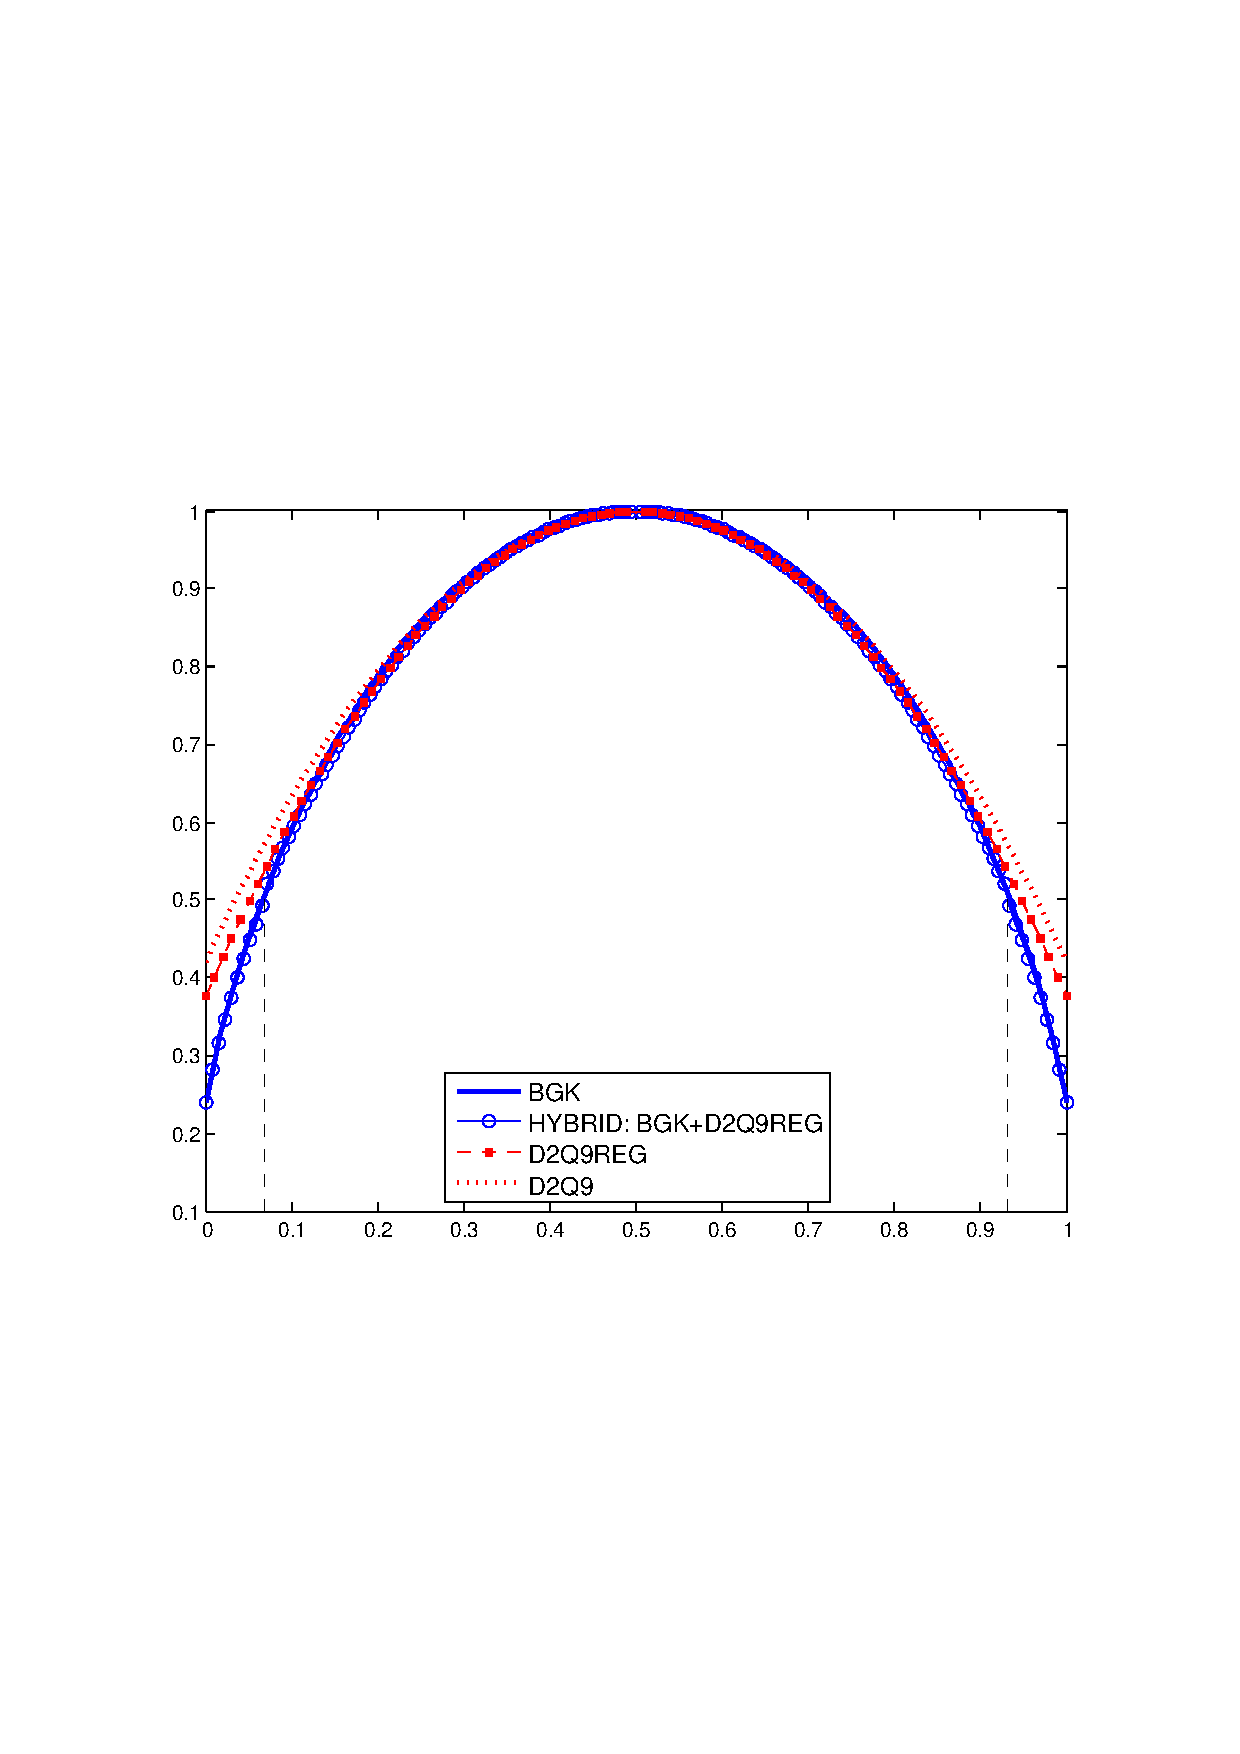
\includegraphics[width=.7\textwidth]{_pois_hybr_kn01_cropped}
    \caption{
        The normalized longitudinal velocity in the linear force-driven Poiseuille flow between parallel plates for $k=0.1$.
        The position of the coupling interface are shown by the vertical dashed lines.
    }\label{fig:poiseuille}
\end{figure}

%%% Poiseuille flow
In addition, the linear Poiseuille-flow problem is solved numerically.
The hybrid solution is compared with the DV and LB ones in Fig.~\ref{fig:poiseuille},
where the D2Q9-regularized LB model is employed~\cite{Latt2006, Mont2015}.
The hybrid solution based on the D2Q9-regularized model is very close to the DV results,
while the D2Q9-regularized model is failed to capture the Knudsen-layer part of the solution.
It is clearly seen from Fig.~\ref{fig:poiseuille} that the application of the regularized LB models in the hybrid scheme
can positively affect the solution accuracy in comparison to the conventional LB models.

\end{comment}

\begin{figure}
    \centering
    \includegraphics{acceleration}
    \caption{
        Computational speed-up yielded by the hybrid method for different CPUs and operational systems.
        $N_0$ is the number of cells in the kinetic zone, $10N_0$ is the number of cells in the bulk region,
        $t_\DV$ and $t_\mathrm{hyb}$ are the total CPU times elapsed by the DV and hybrid methods, respectively.
    }\label{fig:speed-up}
\end{figure}

%%% Efficiency
Finally, let us touch upon the efficiency of the proposed hybrid scheme.
The computational speed-up with respect to the pure DV scheme is shown in Fig.~\ref{fig:speed-up} as a ratio of the corresponding CPU times,
while the ratio of cells in the kinetic and bulk regions remains constant.
One can see that efficiency of the hybrid method achieves the optimum value when number of cells in the kinetic region is more than $10^2$.
Note that the asymptotic speed-up can be slightly higher than the optimum one (12--13 versus 11 in Fig.~\ref{fig:speed-up}).
It is mainly due to memory saving, which results in fewer cache misses.

\section{Conclusion}\label{sec:summary}

%%% What have we done?
In this paper, we have presented a new algorithm for coupling of the DV numerical solutions of the BGK kinetic equation.
The mapping method is based on the Hermite expansion of the VDF.
For the continuum region, we have employed various Gauss--Hermite LB models with different numbers of discrete velocities ranging from 9 to 121.
Incorporating the augmented~\cite{Feuchter2016} LB models % [POISEUILLE]: and regularized~\cite{Latt2006, Mont2015}
positively affect the solution accuracy in comparison to the conventional LB models.
Additional correction procedures have been applied to ensure conservative properties of the hybrid algorithm.
The influence of the breakdown criterion on accuracy and efficiency has also been studied.
The regularized high-order LB models for the hybrid schemes are of interest for further study.

%%% Adaptive mesh in velocity space
A number of problems can be addressed through further study.
A significant number of discrete velocities used for approximation of the VDF is somewhat overkill,
since the highest moments are unimportant for many flows.
Therefore, adaptation of the DV set according to the local flow regime provides room for improving the efficiency of numerical methods
and can serve as a foundation of hybrid schemes for compressible flows.
This approach is similar to the adaptive schemes in velocity space~\cite{Aristov1977, Kolobov2013, Baranger2014}.
%%% Ilyin: applicability of our method
The present scheme can be extended to non-negligible $\Ma$ flows. Since the applied high-order LB model reproduces isothermal hydrodynamics exactly, the method can be applicable to the flows with $\Ma \sim 0.1-0.3$.

%%% Other LB models
The other LB models (e.g., for supersonic flows, compressible and thermal flows~\cite{Chen2010, Frapolli2015, Frapolli2016})
can be incorporated in the proposed hybrid method.
The entropic models are promising due to their enhanced stability for low viscosities (large Reynolds numbers).

% We emphasize that LB is less computationally demanding than DV method. On the other hand, conventional LB is aimed to reproduce only the lowest moments of VDF in slow regimes whereas DV is able to cope with strong nonequilibrium effects.

\section*{Acknowledgements}

This work was supported by the Russian Foundation for Basic Research (Grants 18-01-00899, 18-07-01500).
The authors are grateful to Victor Ambru\textcommabelow{s}, whose comments helped to improve the final version of the manuscript.

\appendix

\section{Third-order TVD limiter}\label{sec:limiter}
...

\section*{References}

\bibliography{dvm-lbm}

\end{document}
